\newpage
\section{Controle}
Todo sistema que trabalha com parâmetros críticos, precisa ser monitorado e controlado de uma forma que o sistema possa manter sua funcionalidade e integridade por mais tempo.
Sendo assim, considerando parâmetros cruciais dentro de um sistema de arrefecimento como temperatura, fluxo e pressão, 
o objetivo da equipe de Controle foi de mostrar uma proposta para o sistema de monitoramento e controle de tal sistema de arrefecimento considerando os âmbitos funcionais e financeiros, 
procurando encontrar a solução mais eficiente e funcional que o mercado possa oferecer.
\subsection{Comparação das propostas}
Houveram duas ideias iniciais que giravam em torno dos sensores de temperatura para a realização do monitoramento dos parâmetros críticos: a primeira delas era focar em um sensor de temperatura que iria ser posicionado juntamente ao sensor 
de pressão da Kistler o qual deve ser resfriado (proposta 1, sistema externo). 
Já a segunda ideia focaria em dois sensores mais baratos que seriam colocados um no 
reservatório e outro na tubulação de saída do sensor de pressão da Kistler e a diferença 
entre eles daria uma noção da temperatura geral do sistema e o quanto este deve ser 
resfriado (proposta 2, sistema interno).

Após melhor análise e estudo do problema, decidiu-se unir as duas propostas em uma só, criando uma terceira proposta que juntasse o melhor das duas.
Dessa forma, essa nova proposta consistiria em um projeto com três sensores de temperatura: um mais próximo do sensor de pressão da Kistler, um na tubulação de saída do próprio sensor e outro no reservatório do líquido, além dos outros sensores de pressão, nível e fluxo.

O diferencial da proposta final está no foco dado à cada sensor em diferentes períodos do teste do foguete híbrido. Durante a realização do teste, os sensores de temperatura internos (localizados no reservatório e na tubulação) serão analisados com maior atenção, a fim de manter a faixa de temperatura no nível de bom funcionamento do sensor de pressão da Kistler. Após o encerramento do teste, o foco principal estará no sensor de temperatura externo (localizado no adaptador da câmara de combustão).
\newpage
\begin{table}[]
    \centering
    \begin{tabular}{|p{3cm}|p{3cm}|p{3cm}|p{3cm}|}
    \hline
    \textbf{ITEM COMPARATIVO} & \textbf{PROPOSTA 1 (Externo)}    & \textbf{PROPOSTA 2 (Interno)} & \textbf{PROPOSTA FINAL (Redundância)}  \\ \hline
    Tipo de mensuração da temperatura no sensor de Pressão da Kistler      & Direta, feita através de um termopar conectado no adaptador do sensor de pressão &  Indireta, feita através da diferença de temperatura entre o sensor do reservatório e o de saída da tubulação &  Combinação das duas propostas, o que resulta em um sistema de redundância e uma escolha de foco na análise dos resultados dependendo da fase de testes  \\ \hline
    Confiabilidade nos dados de medição do parâmetro temperatura & Dependente apenas das informações advindas do sensor no adaptador & Dependente das informações advindas dos sensores na tubulação e no reservatório & Dependente de três sensores de temperatura, o que resulta em um sistema de redundância para este dado \\ \hline
    Flexibilidade em relação à defeitos nos sensores de temperatura & Com apenas um sensor, a suscetibilidade a erros é grande & Com dois sensores dependentes um do outro, a chance de erro é grande & Com um sistema de redundância implementado, as chances de erro diminuem e o sistema pode funcionar de maneira ininterrupta \\ \hline
    Custo total teorizado & Preço comercial de um termopar de qualidade, requer um maior investimento & Preço comercial de um sensor de temperatura simples, acessível & A soma das duas propostas citadas anteriormente \\ \hline
    \end{tabular}
    \caption{Propostas Controle}
    \end{table}

\subsection{Projeto Conceitual}

Considerando então os requisitos necessários para o bom funcionamento do sistema e a proposta definida, foram definidos seis sensores, sendo eles três de temperatura, um de pressão, um de fluxo e um de nível, que serão a porta de entrada de dados e realizarão o monitoramento dos parâmetros cruciais: temperatura, pressão e fluxo. Após diversas pesquisas, os modelos mais adequados para cumprirem essas funções foram:
\newpage
\begin{itemize}
    \item \textbf{Sensor de Temperatura para o adaptador da câmara de combustão}
\end{itemize}
\begin{figure}[!htb]                  
	\centering                          
	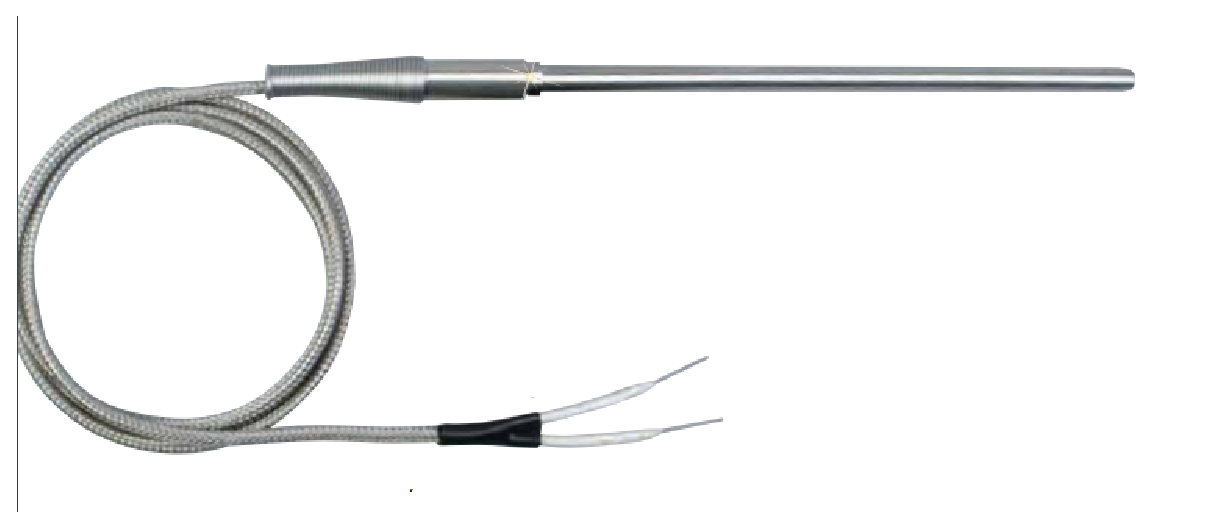
\includegraphics[scale=0.5]{figuras/Sensor1.eps}
	\caption{ Sensor de Temperatura para o adaptador da câmara de combustão }             
\end{figure}

\begin{table}[!h]
    \centering
    \begin{tabular}{|p{5cm}|p{5cm}|p{5cm}|}
    \hline
    \textbf{MODELO} & \textbf{TEMPERATURA}    & \textbf{PREÇO}  \\ \hline
    TJ36-CASS-116G-6-CC-XCIB      & -200 ºC a 899 ºC &  R\$382,00  \\ \hline
    \end{tabular}
    \caption{Sensor de Temperatura para o adaptador da câmara de combustão}
    \end{table}

A escolha deste sensor se deve ao fato principalmente da magnitude da temperatura no adaptador que, por meio de simulações realizadas pelo grupo de transmissão de calor, alcança a faixa de até 450ºC, na posição em que o sensor de pressão principal está localizado. Foi estabelecido um fator de segurança igual a 2, teorizando uma temperatura máxima de 900ºC no adaptador, o que dá maior margem para erros e falhas. Dessa forma, a escolha de um termopar tipo K se justifica, se for considerado a faixa de medição padrão (-200ºC a 1250ºC) e a alta disponibilidade desse tipo de termopar no mercado.

Levando em consideração que os testes realizados no foguete híbrido estão entre 15 e 40 segundos, é necessário que o tempo de resposta dos sensores em geral esteja na escala de milissegundos, a fim de maximizar a coleta de dados e auxiliar na obtenção de resultados dos testes.

Segundo o Manual Técnico de Temperatura da empresa OMEGA, o tempo de resposta de um sensor é o tempo necessário para que um sensor responda a uma mudança de valor na temperatura.
\begin{figure}[!htb]                  
	\centering                          
	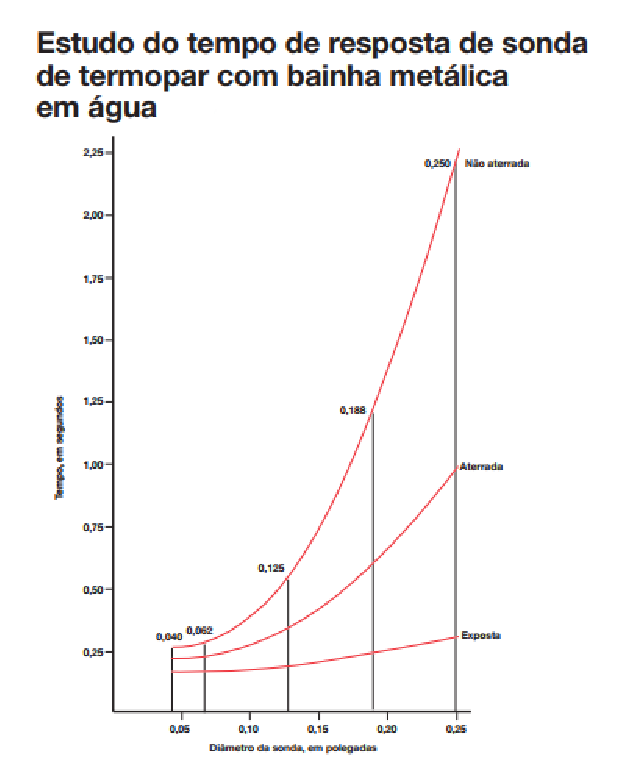
\includegraphics[scale=1.0]{figuras/Figura3.eps}
	\caption{Fonte: Manual Técnico de Temperatura}             
\end{figure}

\newpage

\begin{itemize}
    \item \textbf{Sensor de Temperatura para a tubulação e para o reservatório}
\end{itemize}
\begin{figure}[!htb]                  
	\centering                          
	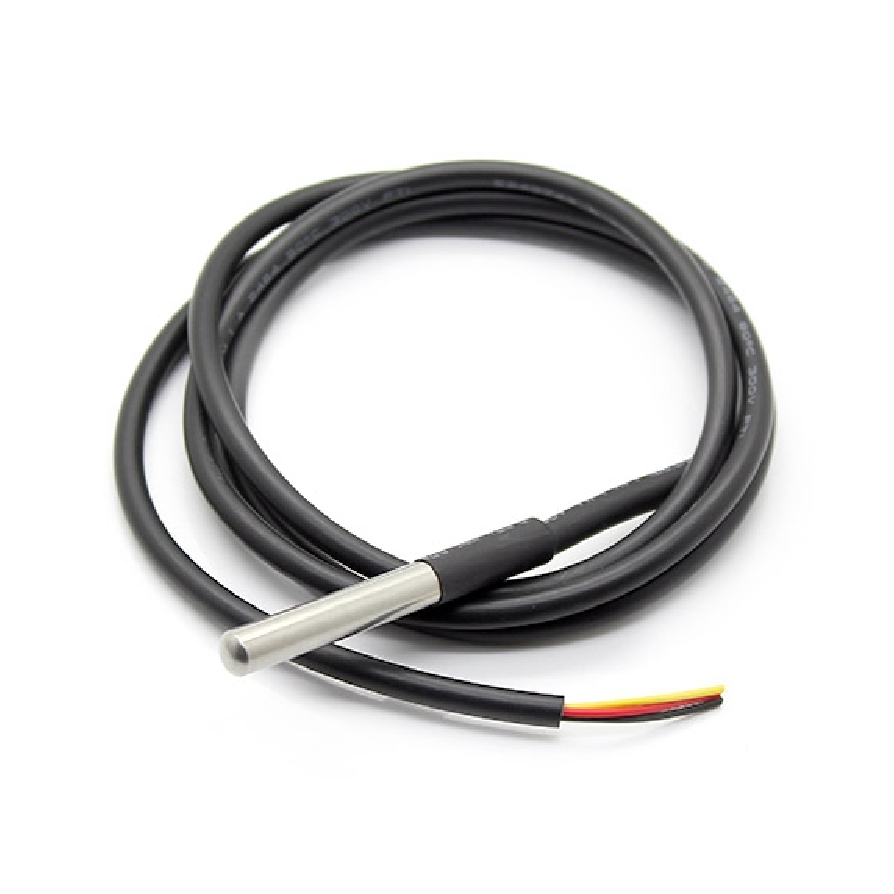
\includegraphics[scale=0.5]{figuras/Figura4.eps}
	\caption{ Sensor de Temperatura para a tubulação e para o reservatório }             
\end{figure}

\begin{table}[]
    \centering
    \begin{tabular}{|p{3cm}|p{5cm}|p{3cm}|p{3cm}|}
    \hline
    \textbf{MODELO} & \textbf{TEMPERATURA}    & \textbf{PREÇO} & \textbf{TEMPO DE RESPOSTA} \\ \hline
    Sensor de Temperatura DS18B20      & -55 ºC até +125 ºC &  R\$16,80 & < que 750 ms  \\ \hline
    \end{tabular}
    \caption{Sensor de Temperatura para a tubulação e para o reservatório}
    \end{table}

Serão utilizados dois sensores deste tipo, um para o reservatório e outro para a tubulação. O sensor que vai no reservatório tem a finalidade de medir a temperatura no local, que segundo estudos do grupo de Transmissão de Calor, deverá estar na faixa de 25 à 30 ºC. A utilização desse sensor é vista como medida de redundância, onde sua principal função é a verificação do funcionamento do sistema de arrefecimento. 

Já o outro sensor, se encontra próximo a tubulação de saída do sensor de pressão da Kistler, com a finalidade de monitorar a temperatura da água na tubulação. Com as simulações do grupo de Transmissão de Calor foi definido que a temperatura do líquido na tubulação de saída será por volta de 90 ºC.

Outros fatores cruciais para a escolha desse sensor para essas duas áreas foram a faixa de medição (que é compatível com as duas localidades), o fato do sensor ser à prova d’água e seu tempo de resposta de menos de 750 ms

\begin{itemize}
    \item \textbf{Sensor de Pressão para a tubulação}
\end{itemize}
\begin{figure}[!htb]                  
	\centering                          
	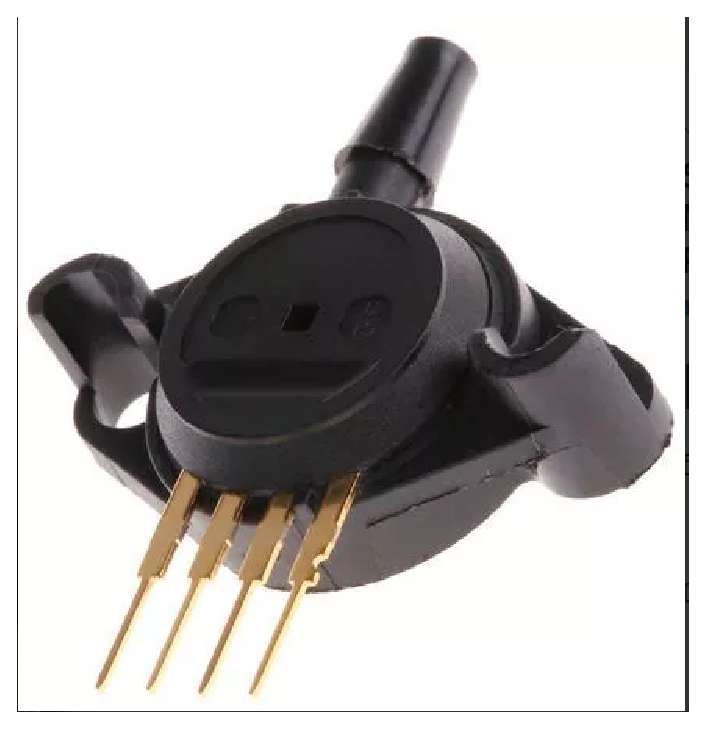
\includegraphics[scale=0.3]{figuras/Figura_5.eps}
	\caption{ Sensor de Pressão para a tubulação}             
\end{figure}

\begin{table}[!h]
    \centering
    \begin{tabular}{|p{3cm}|p{5cm}|p{3cm}|p{3cm}|}
    \hline
    \textbf{MODELO} & \textbf{TEMPERATURA}    & \textbf{PREÇO} & \textbf{TEMPO DE RESPOSTA} \\ \hline
    MPX 2200 GP      & -40 a 125 ºC &  R\$55,00 & 1 ms  \\ \hline
    \end{tabular}
    \caption{Sensor de Pressão para a tubulação}
    \end{table}

A presença desse sensor baseia-se no fato de que um aumento significativo de pressão na tubulação pode gerar um rompimento das conexões, levando ao vazamento da água, e portanto, problemas no sistema de  resfriamento para o sensor.

\begin{itemize}
    \item \textbf{Sensor de Fluxo para a tubulação}
\end{itemize}
\begin{figure}[!htb]                  
	\centering                          
	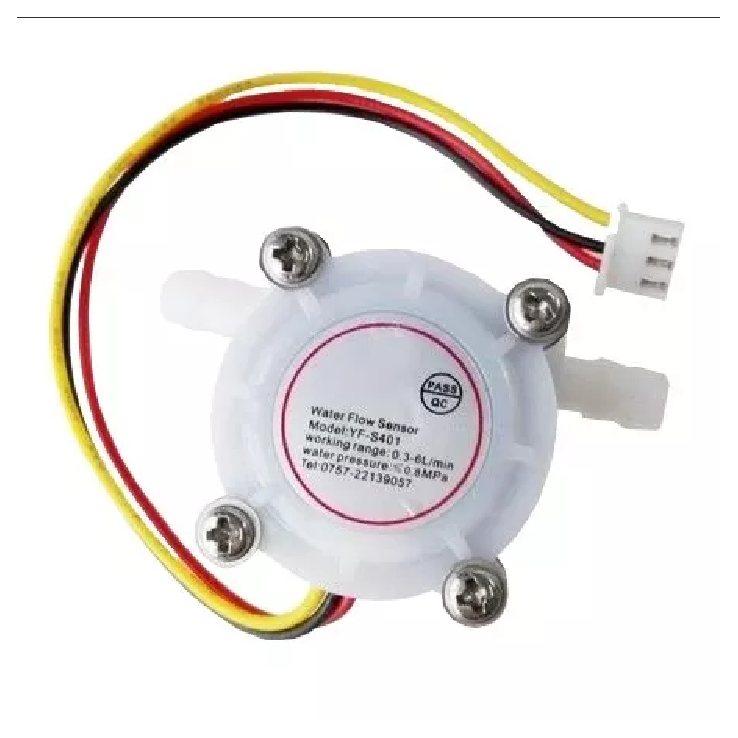
\includegraphics[scale=0.5]{figuras/Figura6.eps}
	\caption{ Sensor de Fluxo para a tubulação}             
\end{figure}

\begin{table}[!h]
    \centering
    \begin{tabular}{|p{3cm}|p{5cm}|p{3cm}|p{3cm}|}
    \hline
    \textbf{MODELO} & \textbf{TEMPERATURA}    & \textbf{PREÇO} \\ \hline
    YF-S401      & até 80 ºC &  R\$28,80  \\ \hline
    \end{tabular}
    \caption{Sensor de Fluxo para a tubulação}
    \end{table}

Este sensor de fluxo ficará posicionado na tubulação do sistema. Seu principal objetivo é monitorar o fluxo do líquido, a fim de acompanhar o funcionamento da bomba d’água. Este sensor servirá como mais um indicativo caso uma falha aconteça no funcionamento da bomba, já que os valores retornados pelo sensor serão fora do esperado, dando pistas sobre qual o possível problema. A escolha deste modelo de sensor de fluxo em específico, se deve a sua ampla utilização no mercado, a sua compatibilidade com diversos microcontroladores existentes.
\newpage
\begin{itemize}
    \item \textbf{Sensor de Nível para o reservatório}
\end{itemize}
\begin{figure}[!h]                  
	\centering                          
	\includegraphics[scale=0.2]{figuras/Figura_7.eps}
	\caption{ Sensor de Nível para o reservatório}             
\end{figure}

\begin{table}[!h]
    \centering
    \begin{tabular}{|p{3cm}|p{5cm}|p{3cm}|p{3cm}|}
    \hline
    \textbf{NOME} & \textbf{TEMPERATURA}    & \textbf{PREÇO} \\ \hline
    Sensor de Nível de Água com Boia Horizontal      & -10 até +85ºC &  R\$24,90  \\ \hline
    \end{tabular}
    \caption{Sensor de Nível para o reservatório}
    \end{table}

A escolha por este sensor é semelhante à escolha do sensor de fluxo. Considerando o local onde será instalado, suas dimensões se adequam às dimensões do reservatório escolhido para guardar o líquido de arrefecimento, além de possuir compatibilidade com Arduino, PIC, ARM, AVR, dentre outras plataformas de prototipagem.

Cabe ressaltar que o uso de um sensor de nível para o reservatório é imprescindível, pois caso ocorra um vazamento, a leitura de dados indicará um problema, visto que se trata de um sistema fechado.

\subsection{Projeto Detalhado}

\begin{itemize}
    \item \textbf{Circuito Amplificador}
\end{itemize}

O grupo de controle determinou 5 sensores para o projeto do sistema de arrefecimento, assim é necessário analisar a necessidade de amplificação de sinais para a correta conectividade com a placa NI6320, que por sua vez aceita apenas sinais de tensão entre 0,2 e 10 Volts, visando assim ter uma maior confiabilidade nos dados transmitidos pelo sensor.
A tabela abaixo determina, para cada sensor a tensão:

\begin{table}[]
    \centering
    \begin{tabular}{|p{3cm}|p{5cm}|p{3cm}|p{3cm}|}
    \hline
    \textbf{\#} & \textbf{Nome}    & \textbf{Modelo} & \textbf{Tensão de saída} \\ \hline
    1      & Sensor de pressão & MPX2200GP  & (-1mV, 40mV)  \\ \hline
    2 & Sensor de temperatura & DS18B20 & (0.5V, 4.5V) \\ \hline
    3 & Sensor de temperatura & TJ36-CASS-116G-6-CC-XCIB & (-6.5mV, -48.8mV) \\ \hline
    4 & Sensor de fluxo & YF-S401 & (4.5V) \\ \hline
    5 & Sensor de nível & NÃO ESPECIFICADO & (4.5V) \\ \hline
    \end{tabular}
    \caption{Tensão por sensor}
    \end{table}

De acordo com uma análise detalhada dos Datasheets usados no projeto de arrefecimento, foram determinadas as saídas de cada sensor. A partir dos requisitos da placa de desenvolvimento usada para o desenvolvimento do projeto é possível afirmar que apenas dois sensores necessitam de amplificação do sinal para a leitura correta. Para os sensores 2, 4 e 5 não há necessidade de amplificação dos sinais, já para os sensores 1 e 3 será necessário. 

O sensor 2 (sensor de temperatura DS18B20) providencia de 9 a 12 bits (configuráveis) que representam a temperatura do dispositivo. A informação é enviada do sensor por apenas um fio, ou seja, o sensor se comunica com a placa de forma serial. Portanto, a tensão de saída será do tipo degrau e representa uma comunicação digital com o microprocessador, do tipo nível lógico 0 ou 1. A partir do Datasheet, foi possível identificar que \textit{VLH} (voltagem do logic high - nível lógico alto) é de 4.5V e que \textit{VLL} (voltagem do low logic - nível lógico baixo) é de 0.5V.
Os sensores 4 e 5 são do tipo pulso magnético. O sensor 4 (sensor de fluxo YF-S401) possui uma estrutura similar a uma concha com pás e uma bobina que uma vez que o fluxo passe pelas pás, o mesmo, pela conservação do momento angular, gera movimento nas pás e, a cada pá que passa pela bobina ela, emite um pulso de corrente através de um fio para o microcontrolador. O sensor 5 (sensor de nível) funciona de maneira semelhante, porém, ao invés de um sistema de pás, a bobina gera um pulso cada vez que o fluxo gera empuxo no mecanismo de acionamento. A saída é, também, do tipo lógico, ou seja, 0.5V para \textit{VLL} e 4.5V para \textit{VLH}.

Os sensores 1 e 3 são do tipo divisores de tensão. A saída de tensão está relacionada com a alcance da grandeza medida (Para o sensor 1, pressão. Para o sensor 3, temperatura). A saída do sensor 1 está na faixa entre -1mV e 40mV e a do sensor 3 está na faixa entre -6.5mV e -48.8 mV.
Foi estabelecido que a amplificação dos sinais utilizará a faixa de 0,2 a 5V, logo é imprescindível o uso de amplificadores instrumentais. Estes conseguem amplificar a tensão e mudar a sua faixa de atuação. A tabela a seguir determina a transição de faixas de tensão que será feita pelos amplificadores:

\begin{table}[]
    \centering
    \begin{tabular}{|p{3cm}|p{5cm}|p{3cm}|p{3cm}|}
    \hline
    \textbf{\#} & \textbf{Sensor}    & \textbf{Tensão de saída regular} & \textbf{Tensão de saída amplificada} \\ \hline
    1      & MPX2200GP & -1mV ~ 40mV   & 1V ~ 5V  \\ \hline
    2 & TJ36-CASS-116G-6-CCXCIB & -6,5mV ~ -48,8mV & 1V ~ 5V \\ \hline
    \end{tabular}
    \caption{Transição de faixas por amplificadores}
    \end{table}

O projeto de amplificação dos sinais utilizou o seguinte amplificador instrumental com os amplificadores operacionais LT071 que possuem pouca distorção de amplificação e podem ser encontrados facilmente no mercado.

\begin{figure}[!h]                  
	\centering                          
	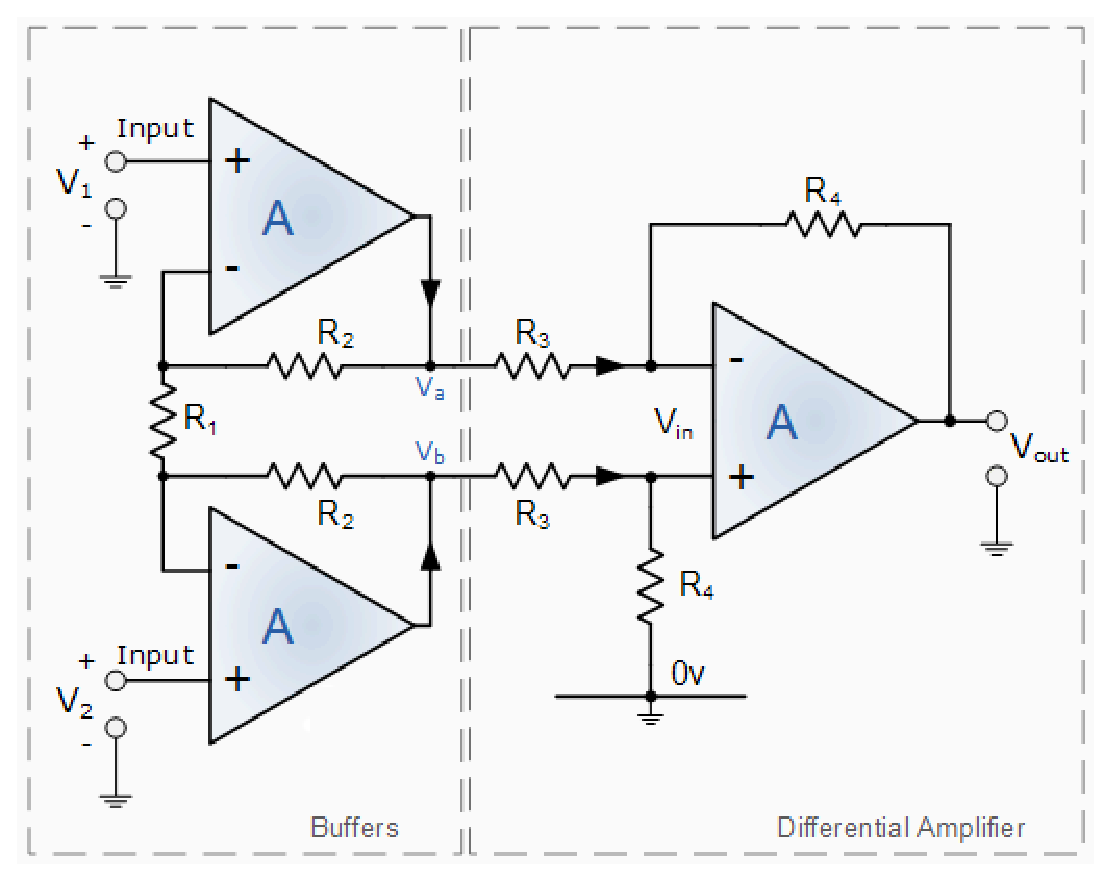
\includegraphics[scale=0.5]{figuras/IMG1.eps}
	\caption{ Amplificador instrumental}             
\end{figure}

A equação que relaciona a tensão de saída e a de entrada é dada pela seguinte expressão:
\begin{equation}\label{eq1tc}
    V_{out}=2*(\frac{R2}{R1})*(\frac{R4}{R3})*(V2-V1)
\end{equation}

O sensor 3 possui tensões de saída negativas, então ele será conectado a \textit{V1} para ser invertido. Já o sensor 1 possui tensões em maioria positivas, logo ele será conectado a \textit{V2}. Este cuidado é necessário para que não seja necessário o uso de resistências negativas no projeto.
Segue abaixo o desenvolvimento das expressões para determinar os resistores e a tensão auxiliar dos dois circuitos de amplificação instrumental.
\newpage
\begin{itemize}
    \item \textbf{Circuito Sensor 1 (Sensor de Pressão)}
\end{itemize}

\begin{equation}\label{eq1tc}
    \alpha = 2*(\frac{R2}{R1})*(\frac{R4}{R3})
\end{equation}
\begin{equation}\label{eq1tc}
    V1 = V_{aux}; V2 = V_{in}
\end{equation}
\begin{equation}\label{eq1tc}
    V_{out} = \alpha[V_{in} - V_{out}]
\end{equation}
\begin{equation}\label{eq1tc}
    5 = \alpha[40 * 10^{-3} - V_{aux}]; 1 = \alpha[-1 * 10^{-3} - V_{aux}]
\end{equation}
\begin{equation}\label{eq1tc}
    \frac{5}{\alpha} = 40 * 10^{-3} - V_{aux}; \frac{1}{\alpha} = -1 * 10^{-3} - V_{aux}
\end{equation}
\begin{equation}\label{eq1tc}
    \frac{5}{\alpha} = 40 * 10^{-3} - V_{aux}; \frac{-1}{\alpha} = 1 * 10^{-3} + V_{aux}
\end{equation}
\begin{equation}\label{eq1tc}
    \frac{4}{\alpha} = 41 * 10^{-3}
\end{equation}

Portanto $\alpha$ = 97,5609756097561.

\(V_{aux}\) = 11,25 mV.

Como $\alpha$ = 2 * \(\frac{R2}{R1}\), então precisamos escolher resistores comerciais que consigam chegar aproximadamente ao valor de $\alpha$, logo a escolha resultou nos resistores:

\begin{equation}\label{eq1tc}
    R2 = (910k\omega + 56k\omega + 9100\omega + 390\omega + 120\omega)
\end{equation}

\begin{equation}\label{eq1tc}
    R1 = (18k\omega + 1k\omega + 1k\omega)
\end{equation}

\begin{equation}\label{eq1tc}
    R4 = R3 = 100k\omega
\end{equation}

Desta forma, segue abaixo o circuito projetado e simulado, no software Proteus 8 Professional:

\begin{figure}[!htb]                  
	\centering                          
	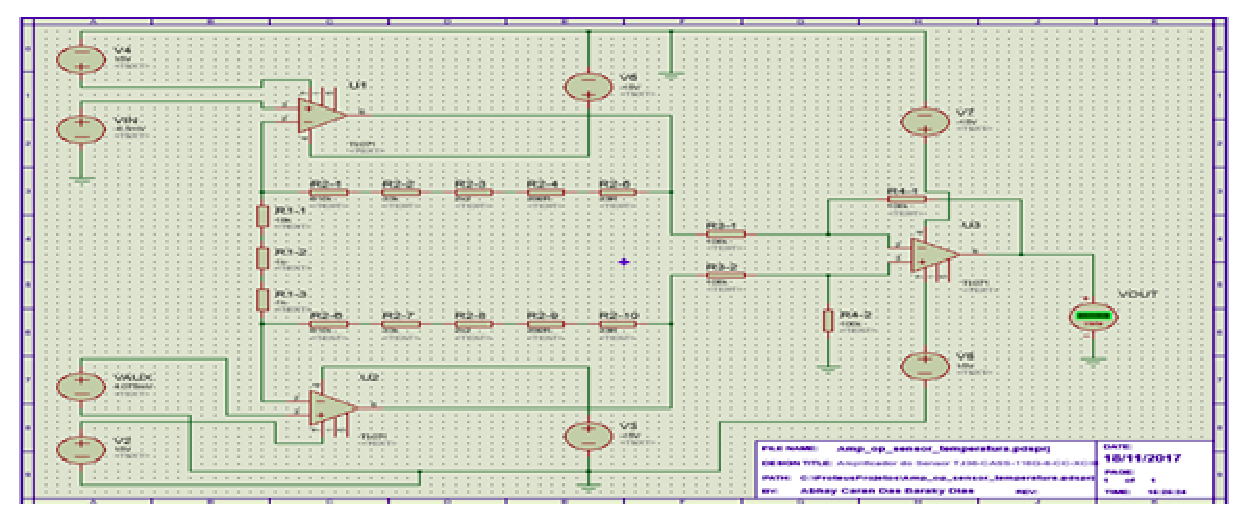
\includegraphics[scale=0.6]{figuras/circ1.eps}
	\caption{ Simulação Circuito Amplificador 2 }             
\end{figure}

\begin{figure}[!htb]                  
	\centering                          
	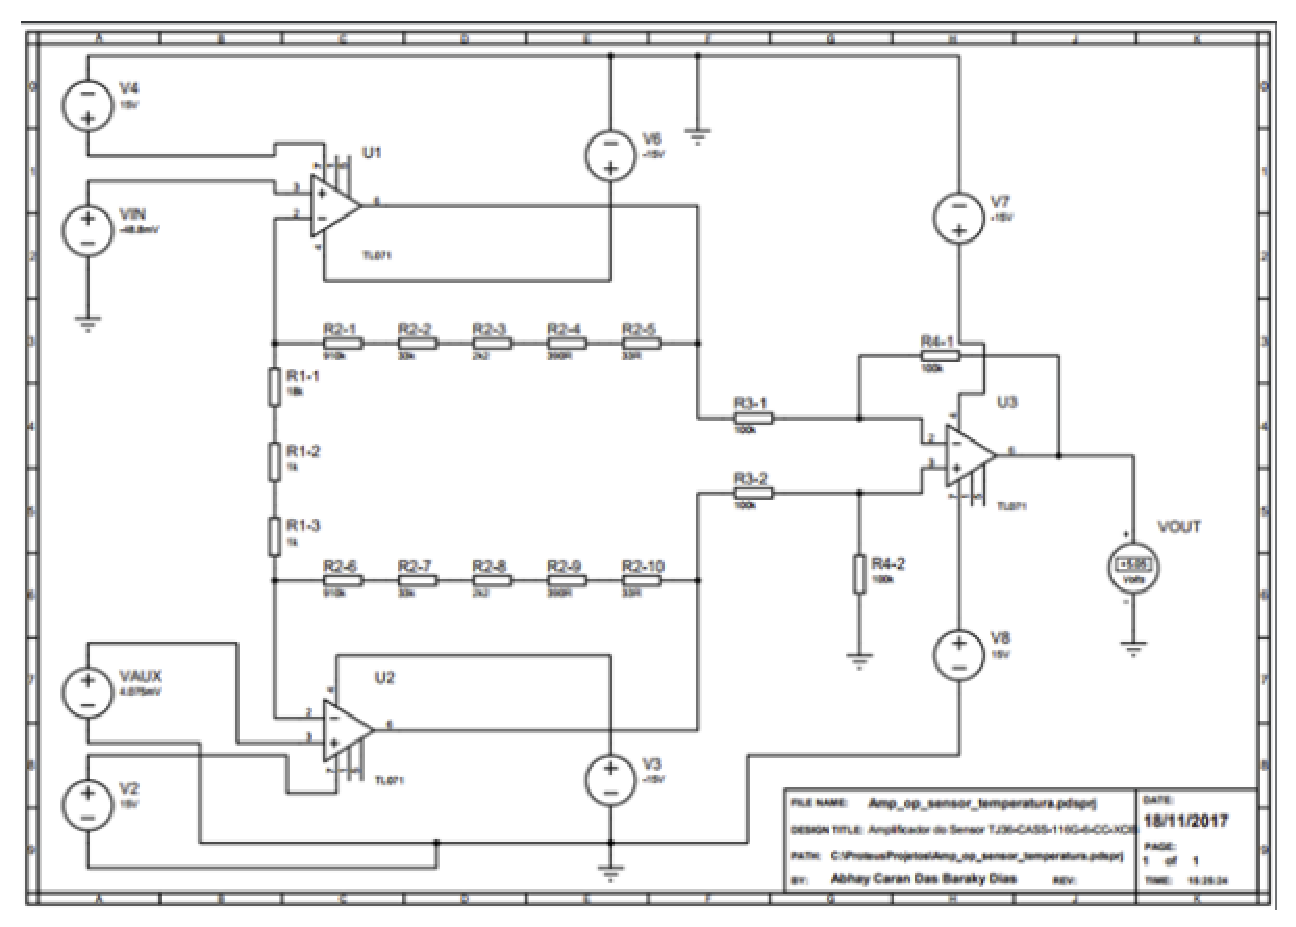
\includegraphics[scale=0.5]{figuras/circ2.eps}
	\caption{ Simulação Circuito Amplificador 2 – Tensão Máxima }             
\end{figure}

\begin{figure}[!htb]                  
	\centering                          
	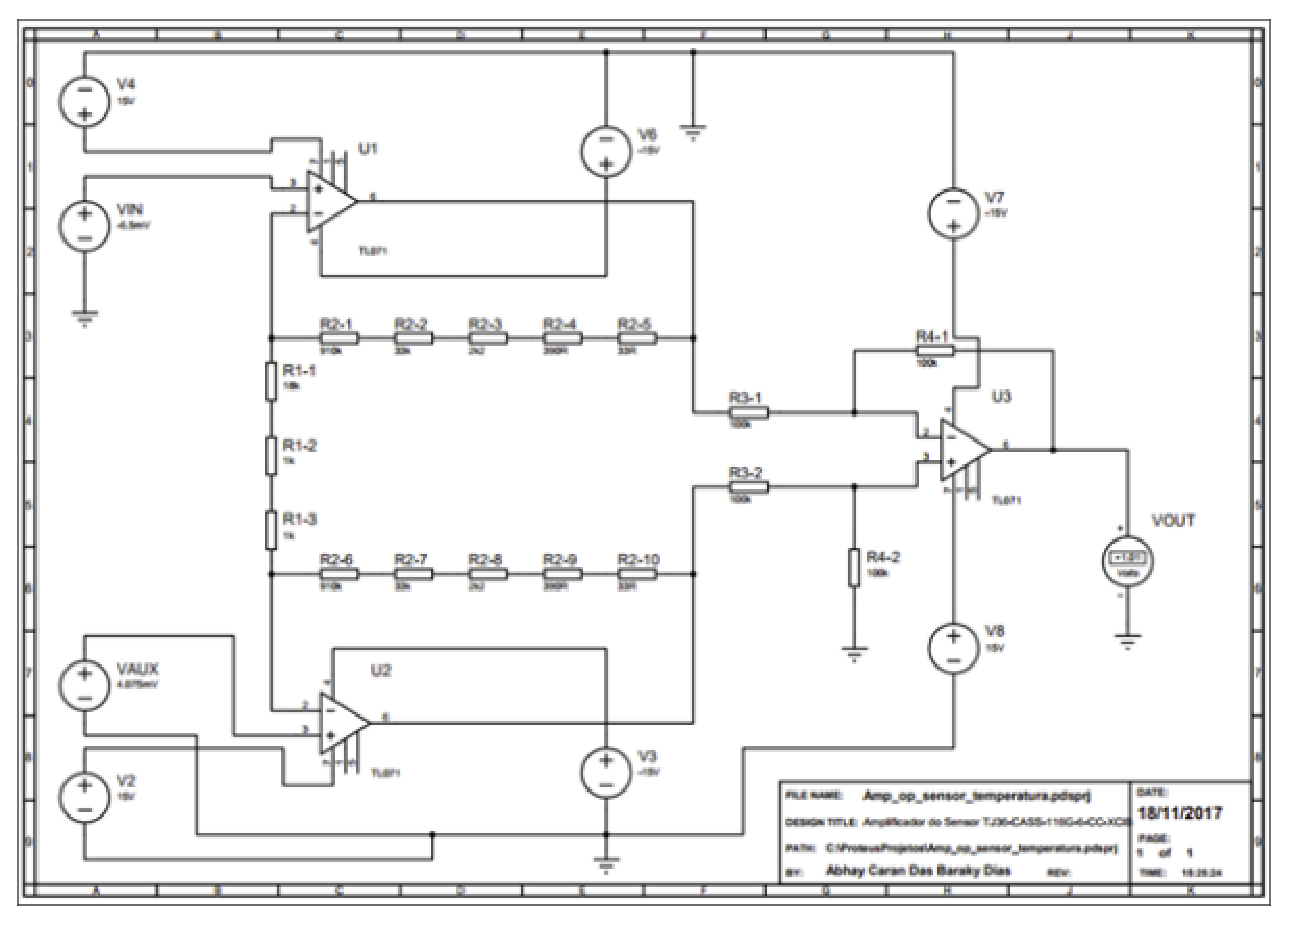
\includegraphics[scale=0.45]{figuras/circ3.eps}
	\caption{ Simulação Circuito Amplificador 2 – Tensão Mínima }             
\end{figure}

